\section[پروژه مسکن کالیفرنیا]{پروژه اول: پیش‌بینی قیمت مسکن کالیفرنیا \\ با پرسپترون (رگرسیون خطی)}

\begin{stepbox}
\field{هدف پروژه}{
در این پروژه، یک مدل رگرسیون خطی ساده (معادل یک پرسپترون تک‌لایه) را برای پیش‌بینی قیمت خانه‌های کالیفرنیا پیاده‌سازی کرده‌ایم. هدف اصلی این گزارش، عبور از کدنویسیِ صرف و رسیدن به درک عمیقِ هندسی و ریاضی از مفاهیمی چون ماتریس همبستگی، پیش‌پردازش داده‌ها، گرادیان کاهشی و نمایش سه‌بعدیِ یادگیری ماشین است.
}
\end{stepbox}

\subsection{دلیل عدم استفاده از دیتاست بوستون \lr{(Boston Housing)} و جایگزینی آن}

در نسخه‌های قدیمی‌تر کتابخانه‌ی \lr{scikit-learn}، دیتاست مسکن بوستون (\lr{load\_boston}) به عنوان استاندارد اصلی آموزشی برای مسائل رگرسیون استفاده می‌شد. اما این دیتاست از نسخه $1.2$ به طور کامل حذف شده است. دلایل اصلی این جایگزینی عبارتند از:

\begin{notebox}[چرا دیتاست بوستون منسوخ شد؟]
\begin{itemize}
    \item \textbf{مسائل اخلاقی و تورش نژادی (\lr{Ethical Bias}):} یکی از ویژگی‌های دیتاست بوستون (متغیر \lr{B}) درصد جمعیت سیاه‌پوست محله را اندازه‌گیری می‌کرد و به طور مستقیم بر فرض ارزان‌تر بودن قیمت خانه بر اساس نژاد دامن می‌زد.
    \item \textbf{قدیمی بودن داده‌ها:} داده‌های بوستون متعلق به سرشماری سال ۱۹۷۰ بودند و ساختارهای اقتصادی جدید را منعکس نمی‌کردند.
\end{itemize}
بنابراین، کتابخانه‌ی \lr{scikit-learn} دیتاست مسکن کالیفرنیا (\lr{fetch\_california\_housing}) را که بر اساس سرشماری ۱۹۹۰ تهیه شده، بدون ویژگی‌های تبعیض‌آمیز است و تعداد نمونه‌های بسیار بیشتری ($20640$ خانه) دارد، به عنوان استاندارد اخلاقی و مدرن جایگزین نمود.
\end{notebox}

\subsection{۱. تحلیل اکتشافی داده‌ها \lr{(EDA)} و بررسی تفصیلی هیت‌مپ‌ها}

اولین گام، درک رابطه خطی ویژگی‌ها با هدف است. ماتریس همبستگی پیرسون \lr{(Pearson Correlation)} به صورت زیر تعریف می‌شود:
\[
r = \frac{\sum (x_i - \bar{x})(y_i - \bar{y})}{\sqrt{\sum (x_i - \bar{x})^2 \sum (y_i - \bar{y})^2}}
\]

در ادامه، هر یک از ۳ هیت‌مپ خروجی کد به همراه تحلیل دقیق هندسی آورده شده است:

\subsubsection{۱-۱. ماتریس کامل همبستگی تمامی ویژگی‌ها}

\begin{figure}[htbp]
    \centering
    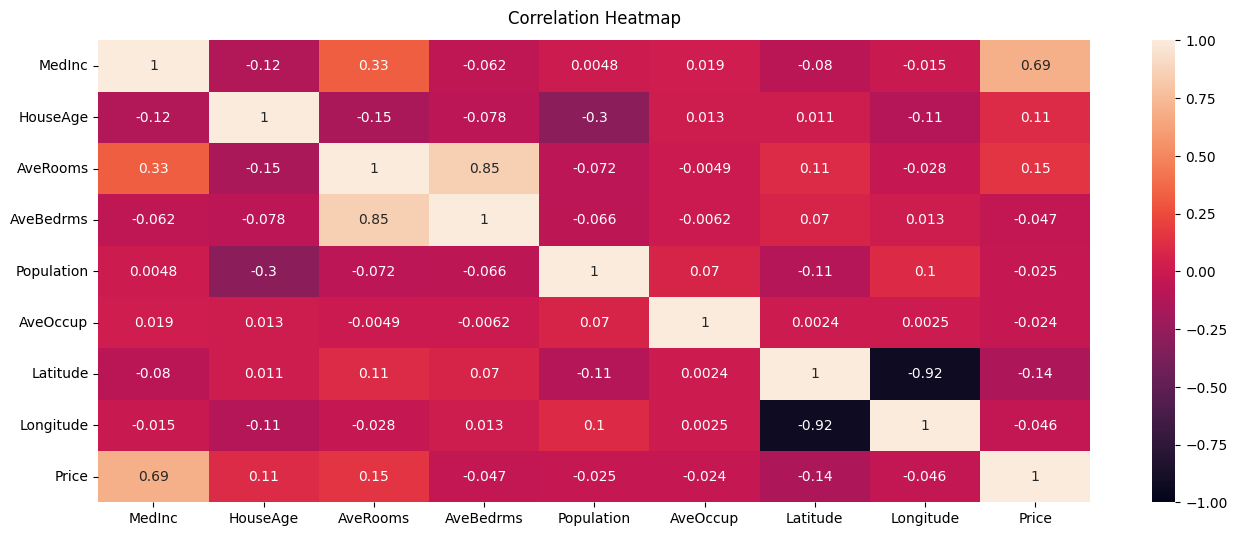
\includegraphics[width=0.60\textwidth]{images/img_corr_full.png}
    \caption{نقشه حرارتی (\lr{Heatmap}) ماتریس همبستگی کامل تمامی ویژگی‌های دیتاست کالیفرنیا.}
    \label{fig:corr_full}
\end{figure}

\noindent \textbf{تحلیل ماتریس کامل:}
بررسی کامل این ماتریس به ما کمک می‌کند تله‌های ریاضی را شناسایی کنیم:
\begin{itemize}
    \item \textbf{تله هم‌خطی چندگانه (\lr{Multicollinearity}):} همبستگی بین \lr{AveRooms} و \lr{AveBedrms} برابر با $0.85$ است. انتخاب همزمان این دو ویژگی مدل را دچار سردرگمی شدید کرده و نوسانات ناپایدار در وزن‌ها ایجاد می‌کند.
    \item \textbf{همبستگی جغرافیایی:} طول و عرض جغرافیایی (\lr{Latitude} و \lr{Longitude}) همبستگی منفی $-0.92$ دارند که نشان‌دهنده مورب بودن ساختار جغرافیایی ایالت کالیفرنیاست.
\end{itemize}

\subsubsection{۱-۲. همبستگی ویژگی‌ها با متغیر هدف و ویژگی اصلی}

\begin{figure}[htbp]
    \centering
    \begin{subfigure}{0.48\textwidth}
        \centering
        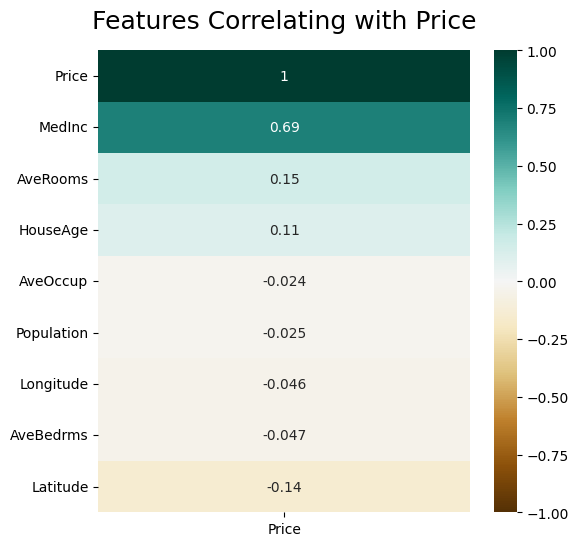
\includegraphics[width=0.75\textwidth]{images/img_corr_price.png}
        \caption{همبستگی با متغیر هدف (\lr{Price})}
        \label{fig:corr_price}
    \end{subfigure}
    \hfill
    \begin{subfigure}{0.48\textwidth}
        \centering
        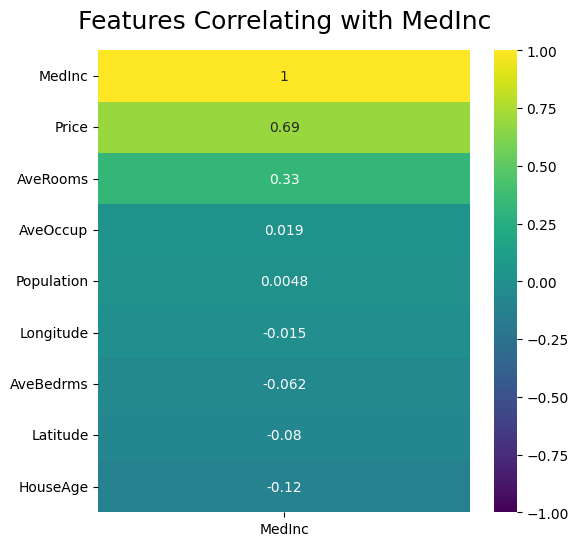
\includegraphics[width=0.75\textwidth]{images/img_corr_medinc.png}
        \caption{همبستگی با متغیر اصلی (\lr{MedInc})}
        \label{fig:corr_medinc}
    \end{subfigure}
    \caption{بررسی ستون‌های همبستگی جهت انتخاب ۲ ویژگی ورودی به پرسپترون.}
    \label{fig:corr_side_by_side}
\end{figure}

\noindent \textbf{تحلیل ستون هدف و استقلال ویژگی دوم:}
\begin{itemize}
    \item \textbf{قوی‌ترین سیگنال خطی (\lr{MedInc}):} ویژگی درآمد متوسط محله (\lr{MedInc}) با ضریب $0.69$ بالاترین همبستگی مثبت مستقیم با قیمت دارد و به عنوان متغیر ورودی اول ($x_1$) انتخاب شد.
    \item \textbf{استقلال ویژگی دوم (\lr{HouseAge}):} برای انتخاب ویژگی دوم ($x_2$)، به دنبال متغیری بودیم که با $x_1$ همبستگی نزدیک به صفر داشته باشد. ویژگی \lr{HouseAge} همبستگی $0.11$ با قیمت دارد و همبستگی آن با \lr{MedInc} برابر با $-0.12$ است. این استقلال اطلاعاتی باعث شد \lr{HouseAge} به عنوان ویژگی دوم انتخاب شود.
\end{itemize}

\subsection{۲. پیش‌پردازش داده‌ها \lr{(Data Preprocessing)}}

پیش از ورود داده‌ها به شبکه‌ی عصبی، آن‌ها را با نسبت ۸۰ به ۲۰ به داده‌های آموزش و تست تقسیم کردیم. سپس مقیاس‌بندی ویژگی‌ها انجام شد.

\begin{warnbox}[اهمیت استانداردسازی در \lr{PyTorch}]
ویژگی درآمد اعدادی کوچک (بین ۱ تا ۱۵) و ویژگی سن خانه اعدادی بزرگ‌تر (تا ۵۰) داشت. اگر داده‌ها به همین شکل وارد مدل می‌شدند، الگوریتم بهینه‌ساز (\lr{Gradient Descent}) در یک فضای بیضوی و ناهموار گرفتار می‌شد و گرادیان‌ها واگرا می‌شدند.
\end{warnbox}

با استفاده از \lr{\texttt{StandardScaler}}، داده‌ها را به توزیعی با میانگین ۰ و واریانس ۱ تبدیل کردیم (فرمول $z = \frac{x - \mu}{\sigma}$). در نهایت تمامی داده‌ها از فرمت \lr{Pandas/NumPy} به تنسورهای \lr{PyTorch} با نوع \lr{\texttt{torch.float32}} تبدیل شدند تا گراف محاسباتی بتواند روی آن‌ها تشکیل شود.

\subsection{۳. معماری مدل و ریاضیات}

مدل ما یک ترکیب خطی ساده است که در فضای سه‌بعدی یک صفحه (\lr{Plane}) را می‌سازد. معادلات حاکم بر این شبکه به شرح زیر است:

\textbf{۱. فاز پیش‌رو \lr{(Forward Pass)}:}
\[
\hat{y} = w_1 x_1 + w_2 x_2 + b
\]

\textbf{۲. تابع هزینه \lr{(Loss Function - MSE)}:}
\[
J(W, b) = \frac{1}{N} \sum_{i=1}^{N} (\hat{y}^{(i)} - y^{(i)})^2
\]

\textbf{۳. الگوریتم آپدیت وزن‌ها \lr{(Gradient Descent)}:}
\[
W \leftarrow W - \alpha \frac{\partial J}{\partial W}
\]

\subsection{۴. پیاده‌سازی و آموزش در \lr{PyTorch}}

ما مدل را با استفاده از \lr{\texttt{nn.Linear(2, 1)}} تعریف کرده و از بهینه‌ساز \lr{SGD} با نرخ یادگیری $0.01$ استفاده کردیم. کد حلقه‌ی آموزش در قطعه‌ی زیر قابل مشاهده است:

\begin{codebox}[\texttt{train\_perceptron.py}]
\begin{lstlisting}[language=Python]
epochs = 100
for epoch in range(epochs):
    y_pred = perceptron_linear(X_train)       # Forward pass
    loss = criterion(y_pred, y_train)         # Compute MSE
    optimizer.zero_grad()                     # Clear old gradients
    loss.backward()                           # Autograd (Compute gradients)
    optimizer.step()                          # Update weights
\end{lstlisting}
\end{codebox}

\begin{tipbox}[تله‌ی ابعاد - \lr{Broadcasting}]
یکی از چالش‌های مهم در این بخش، اطمینان از یکسان بودن ابعاد \lr{y\_pred} و \lr{y\_train} بود تا \lr{PyTorch} به اشتباه یک ماتریس $N \times N$ نسازد. پس از رفع این مورد، مقدار خطا (Loss) با شیب بسیار مناسبی از عدد $4.18$ به حدود $0.74$ در اپوک ۱۰۰ کاهش یافت.
\end{tipbox}

\subsection{۵. تحلیل هندسی و بصری‌سازی نتایج}

پس از استخراج وزن‌های نهایی مدل ($w_1 = 0.7928$, $w_2 = 0.2248$, $b = 1.8193$)، عملکرد مدل را از سه زاویه‌ی مختلف بررسی کردیم. توضیحات و تحلیل ریاضی هر نمودار دقیقاً در کنار تصویر مربوطه‌اش قرار گرفته است:

\subsubsection{۵-۱. نمای هندسی سه‌بعدی \lr{(The Hyperplane)}}

\begin{figure}[htbp]
    \centering
    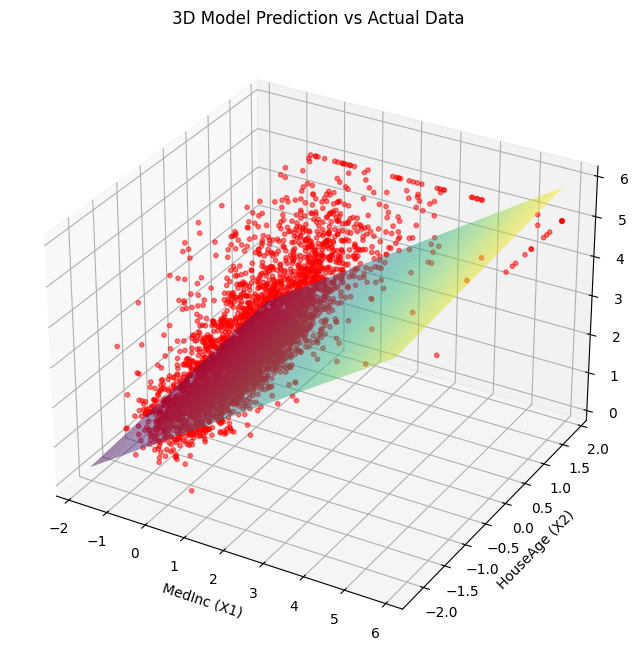
\includegraphics[width=0.50\textwidth]{images/img_3d_plane.png}
    \caption{مدل خطی آموزش‌دیده (صفحه) که از میان ابر نقاط داده واقعی عبور کرده است.}
    \label{fig:3d_plane}
\end{figure}

\noindent \textbf{تحلیل هندسی صفحه ۳ بعدی:}
این نمودار تجسم دقیق معادله‌ی $\hat{y} = w_1 x_1 + w_2 x_2 + b$ است. صفحه مدل ما، بهترین شیب و زاویه را پیدا کرده تا کمترین فاصله را با نقاط واقعی (قرمز) داشته باشد. مثبت بودن وزن‌ها نشان می‌دهد که با افزایش درآمد و سن خانه، قیمت به‌طور خطی بالا می‌رود.

\subsubsection{۵-۲. تحلیل پسماندها \lr{(Residual Analysis)}}

\begin{figure}[htbp]
    \centering
    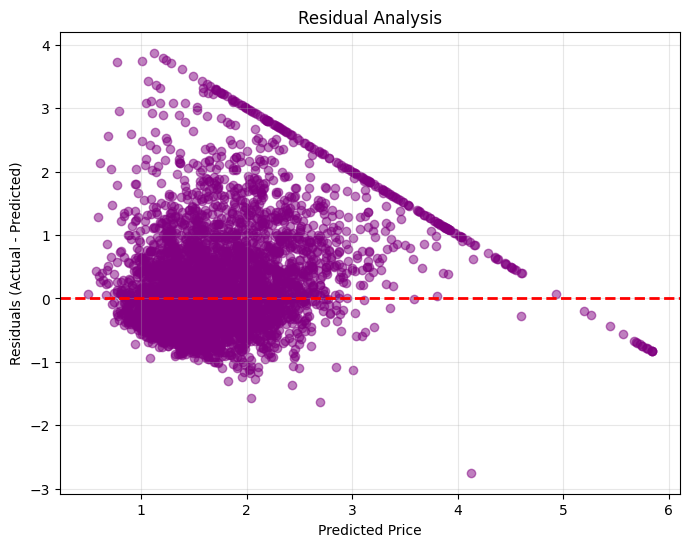
\includegraphics[width=0.45\textwidth]{images/img_residuals.png}
    \caption{توزیع خطاهای مدل نسبت به خط خطای صفر.}
    \label{fig:residuals}
\end{figure}

\noindent \textbf{تحلیل رفتار خطاها (پسماندها):}
این نمودار (نقاط بنفش) خطای پیش‌بینی را نشان می‌دهد. اگر مدل کامل بود، خطاها فقط یک نویز تصادفی حول خط قرمز (صفر) بودند. اما مشاهده‌ی الگو در قیمت‌های بالا نشان می‌دهد که رابطه‌ی قیمت و ویژگی‌ها صددرصد خطی نیست و این مدل برای داده‌های غیرخطی محدودیت دارد.

\subsubsection{۵-۳. برش دو بعدی \lr{(2D Slice - Effect of MedInc)}}

\begin{figure}[htbp]
    \centering
    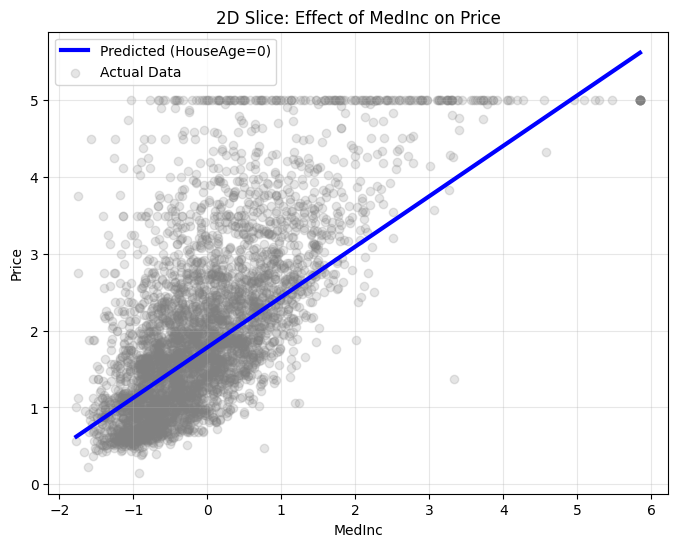
\includegraphics[width=0.45\textwidth]{images/img_2d_slice.png}
    \caption{برش صفحه سه‌بعدی؛ نمایش اثر مستقیم درآمد بر قیمت در صورت ثابت ماندن متغیر سن.}
    \label{fig:2d_slice}
\end{figure}

\noindent \textbf{تحلیل اثر متغیر درآمد در برش ۲ بعدی:}
با صفر در نظر گرفتن متغیر \lr{HouseAge} (معادل قرار دادن آن روی میانگینِ استاندارد شده)، صفحه سه‌بعدی تبدیل به یک خط راست شد. شیب این خط آبی دقیقاً نشان‌دهنده‌ی وزنِ یادگرفته‌شده برای ویژگی درآمد ($w_1 \approx 0.79$) است.
